\documentclass[11pt]{article}
\usepackage[T1]{fontenc}
\usepackage[margin=1in]{geometry}
\usepackage{graphicx}
\usepackage{booktabs}
\usepackage{float}
\usepackage[font=small]{caption}

\newcommand{\cm}[4]{\begin{tabular}{@{}l|cc@{}} & Pred.\ N & Pred.\ P\\ \hline Actual N & #1 & #2\\ Actual P & #3 & #4\end{tabular}}

\title{CPEN 693 -- Homework 2}
\author{}
\date{\today}

\begin{document}
\maketitle

\section{Breast Cancer Classification (Problem 1)}

\subsection*{Method}
Malignant (positive) versus benign (negative) tumours are classified using a support vector machine (SVM) and k-nearest neighbours (kNN). Linear, RBF, polynomial and sigmoid kernels, and $k=1$--$10$, are compared; the best setting for each model is reported.

\subsection*{Implementation Details}
The Wisconsin Diagnostic CSV (569 samples, all 30 features) is split 75/25 (stratified, seed 42). Features are standardized with training-set statistics. scikit-learn's SVC and KNeighborsClassifier use default parameters; the best kernel and $k$ are chosen by test accuracy.

\subsection*{Results}
Across kernels and $k$ (Table~\ref{tab:p1sweep}), RBF-SVM and kNN ($k=7$) both reach the best accuracy, 0.972, with identical confusion matrices (Table~\ref{tab:p1cm}): 90 true negatives, 49 true positives, no false positives, four false negatives. Sensitivity is 0.925 and specificity 1.000. The polynomial kernel is weakest (0.895); kNN accuracy ranges from 0.930 to 0.972.

\begin{table}[H]
\centering
\caption{Test accuracy for each SVM kernel and each kNN $k$ (best in bold).}
\label{tab:p1sweep}
\begin{tabular}{lcccc}
\toprule
SVM kernel & Linear & RBF & Poly. & Sigmoid\\
Accuracy & 0.958 & \textbf{0.972} & 0.895 & 0.951\\
\bottomrule
\end{tabular}

\vspace{6pt}
\begin{tabular}{lcccccccccc}
\toprule
kNN $k$ & 1 & 2 & 3 & 4 & 5 & 6 & 7 & 8 & 9 & 10\\
Accuracy & 0.937 & 0.930 & 0.958 & 0.958 & 0.958 & 0.965 & \textbf{0.972} & 0.965 & 0.958 & 0.958\\
\bottomrule
\end{tabular}
\end{table}

\begin{table}[H]
\centering
\caption{Confusion matrices on the 143 test samples (N = benign, P = malignant), with sensitivity (Sens.), specificity (Spec.) and accuracy (Acc.).}
\label{tab:p1cm}
\begin{tabular}{llcccc}
\toprule
Model & Setting & Confusion matrix & Sens. & Spec. & Acc.\\
\midrule
SVM & RBF kernel & \cm{90}{0}{4}{49} & 0.925 & 1.000 & 0.972\\
kNN & $k=7$ & \cm{90}{0}{4}{49} & 0.925 & 1.000 & 0.972\\
\bottomrule
\end{tabular}
\end{table}

\section{EEG Seizure Detection (Problem 2)}

\subsection*{Method}
The variance of each EEG recording is the only feature. SVM and kNN separate A (healthy) vs D (seizure-free), A vs E (seizure) and D vs E; the second set of each pair is the positive class. Kernels and $k$ are compared as before.

\subsection*{Implementation Details}
Sets A, D and E (Bonn dataset, 100 recordings of 4097 samples each) are loaded; one recording per set is plotted (Figure~\ref{fig:eeg}). The 200 variance values per pair are split 75/25 (stratified) and standardized. SVC and KNeighborsClassifier are tuned by test accuracy.

\subsection*{Results}
Set E is separated easily: kNN ($k=1$) classifies A vs E perfectly and RBF-SVM reaches 0.980. D vs E reaches 0.920 with both models. A vs D is hardest (kNN 0.720, SVM 0.640), indicating strong variance overlap between healthy and interictal recordings. SVM favours specificity there (sensitivity 0.280). Full confusion matrices are in Table~\ref{tab:p2cm}.

\begin{figure}[H]
\centering
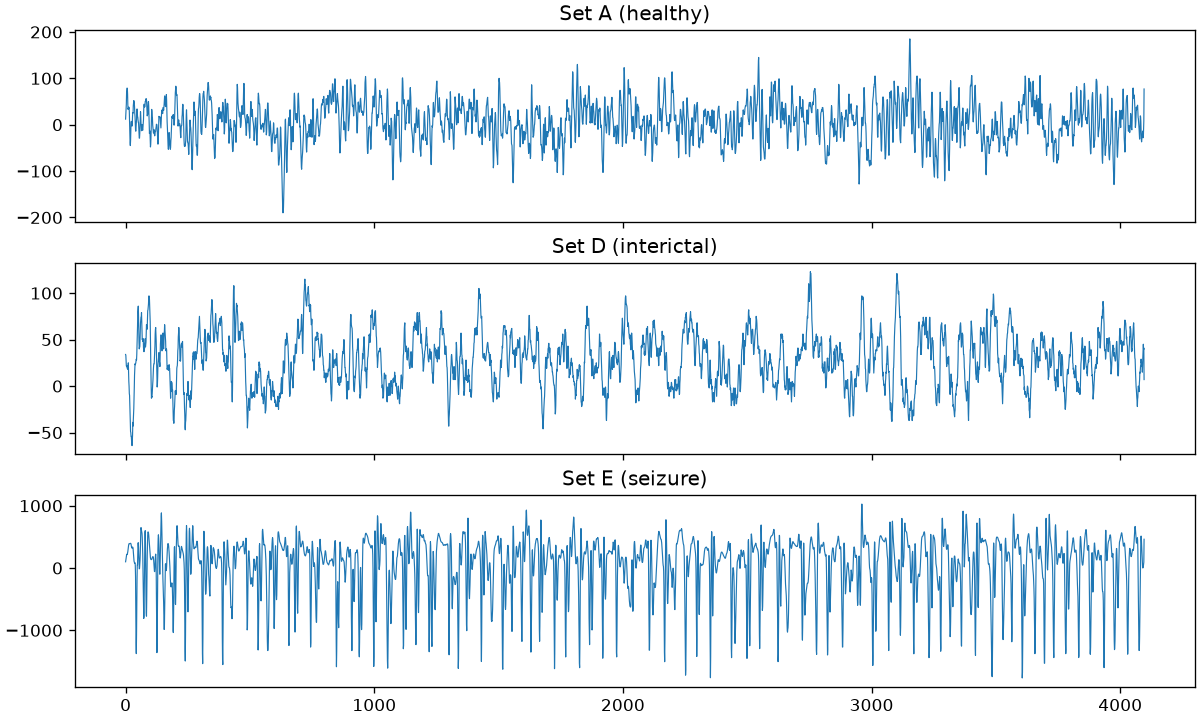
\includegraphics[width=\linewidth]{figures/problem2_eeg_samples.png}
\caption{One EEG recording from each set: A (healthy), D (seizure-free interictal) and E (seizure attack).}
\label{fig:eeg}
\end{figure}

\begin{table}[H]
\centering
\caption{Confusion matrices on the 50 test samples per task (N = first set, P = second set), with sensitivity (Sens.), specificity (Spec.) and accuracy (Acc.).}
\label{tab:p2cm}
\begin{tabular}{lllcccc}
\toprule
Task & Model & Setting & Confusion matrix & Sens. & Spec. & Acc.\\
\midrule
A vs D & SVM & RBF kernel & \cm{25}{0}{18}{7} & 0.280 & 1.000 & 0.640\\
 & kNN & $k=10$ & \cm{22}{3}{11}{14} & 0.560 & 0.880 & 0.720\\
\midrule
A vs E & SVM & RBF kernel & \cm{25}{0}{1}{24} & 0.960 & 1.000 & 0.980\\
 & kNN & $k=1$ & \cm{25}{0}{0}{25} & 1.000 & 1.000 & 1.000\\
\midrule
D vs E & SVM & Linear kernel & \cm{23}{2}{2}{23} & 0.920 & 0.920 & 0.920\\
 & kNN & $k=2$ & \cm{22}{3}{1}{24} & 0.960 & 0.880 & 0.920\\
\bottomrule
\end{tabular}
\end{table}

\section{MNIST Classification (Problem 3)}

\subsection*{Method}
A fully connected network maps the flattened 28$\times$28 image (Figure~\ref{fig:p3samples}) to ten digit classes. Depth (one to six hidden layers), width, activation (ReLU, Tanh) and dropout (0, 0.2) are varied. Weight decay and early stopping limit overfitting; configurations are selected by validation accuracy.

\subsection*{Implementation Details}
55k training, 5k validation (held out from the 60k training set) and 10k test images; pixels in [0,1]. AdamW (learning rate $10^{-3}$, weight decay 0.01), batch size 128, at most 50 epochs, RTX 5080 GPU. Early stopping (patience 5) monitors validation loss; only the selected model is tested.

\subsection*{Results}
The six-layer ReLU network with dropout 0.2 has the highest validation accuracy (0.9828) and is selected; its test accuracy is 0.9810, with 17.0 s training time (Table~\ref{tab:p3}). Early stopping ended runs after 10--23 epochs (Figure~\ref{fig:p3loss}). Dropout helped the five-layer network (validation 0.9762 to 0.9810). Test accuracy is reported only for the selected network.

\begin{figure}[H]
\centering
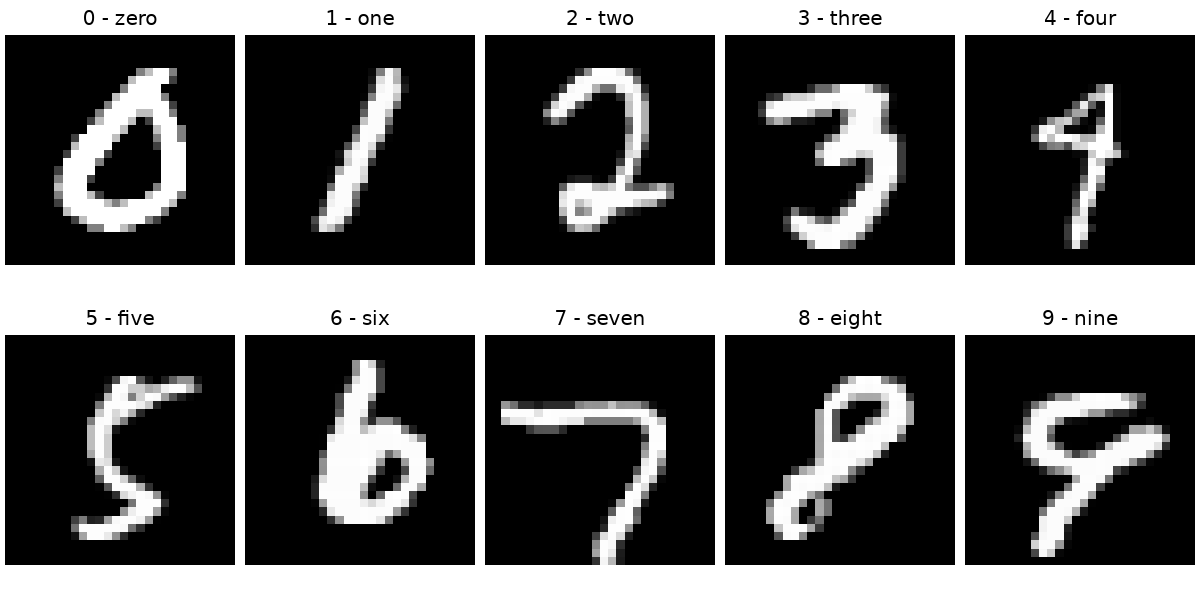
\includegraphics[width=0.85\linewidth]{figures/problem3_samples.png}
\caption{One training image from each MNIST digit class.}
\label{fig:p3samples}
\end{figure}

\begin{figure}[H]
\centering
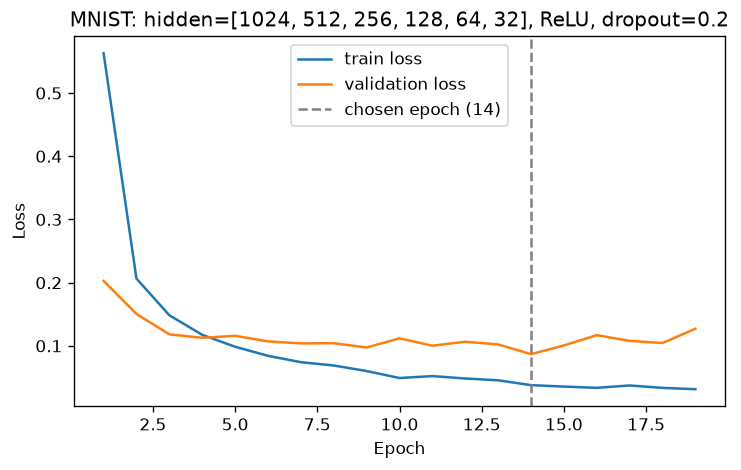
\includegraphics[width=0.7\linewidth]{figures/problem3_loss.png}
\caption{Training and validation loss versus epoch for the selected MNIST network. The dashed line marks the chosen epoch 14, whose weights are kept; early stopping ended training at epoch 19.}
\label{fig:p3loss}
\end{figure}

\begin{table}[H]
\centering
\caption{MNIST configurations (hidden layer sizes): epochs run before early stopping, training time (including per-epoch validation), validation accuracy and, for the selected network only, test accuracy (selected row in bold).}
\label{tab:p3}
\small
\setlength{\tabcolsep}{4pt}
\begin{tabular}{llccccc}
\toprule
Hidden layers & Activation & Dropout & Epochs & Time (s) & Val. acc. & Test acc.\\
\midrule
128 & ReLU & 0 & 23 & 12.3 & 0.9792 & --\\
256-128 & ReLU & 0 & 13 & 7.8 & 0.9774 & --\\
512-256-128 & ReLU & 0 & 18 & 11.7 & 0.9820 & --\\
256-128 & Tanh & 0 & 13 & 7.8 & 0.9768 & --\\
512-256-128-64 & ReLU & 0.2 & 15 & 11.3 & 0.9798 & --\\
512-512-256-256-128 & ReLU & 0 & 10 & 7.4 & 0.9762 & --\\
512-512-256-256-128 & ReLU & 0.2 & 16 & 13.0 & 0.9810 & --\\
1024-512-256-128-64-32 & ReLU & 0.2 & 19 & 17.0 & \textbf{0.9828} & \textbf{0.9810}\\
\bottomrule
\end{tabular}
\end{table}

\section{Fashion-MNIST Classification (Problem 4)}

\subsection*{Method}
A fully connected network maps the flattened 28$\times$28 image (Figure~\ref{fig:p4samples}) to ten clothing classes. Depth (one to six hidden layers), width, activation (ReLU, Tanh) and dropout (0, 0.2) are varied. Weight decay and early stopping limit overfitting; configurations are selected by validation accuracy.

\subsection*{Implementation Details}
55k training, 5k validation (held out from the 60k training set) and 10k test images; pixels in [0,1]. AdamW (learning rate $10^{-3}$, weight decay 0.01), batch size 128, at most 50 epochs, RTX 5080 GPU. Early stopping (patience 5) monitors validation loss; only the selected model is tested.

\subsection*{Results}
The five-layer ReLU network with dropout 0.2 has the highest validation accuracy (0.8918) and is selected: test accuracy 0.8857, training time 17.1 s (Table~\ref{tab:p4}). Dropout made no measurable difference for this network (0.8916 without). Validation accuracies of all configurations lie within 0.8856--0.8918, and early stopping restored epoch 16 of 21 (Figure~\ref{fig:p4loss}).

\begin{figure}[H]
\centering
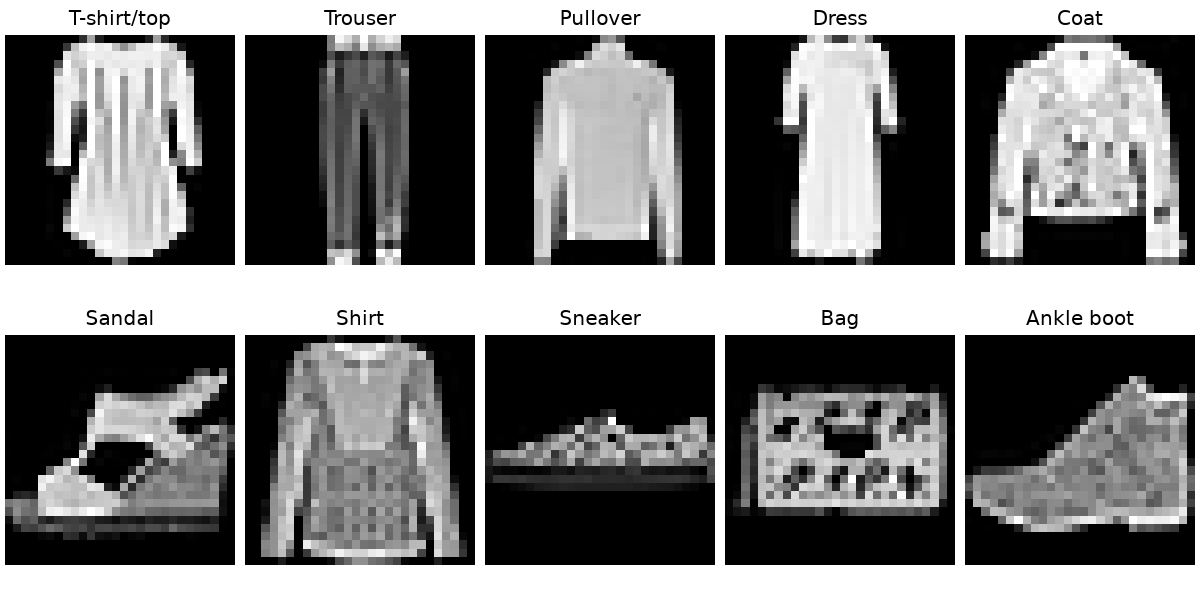
\includegraphics[width=0.85\linewidth]{figures/problem4_samples.png}
\caption{One training image from each Fashion-MNIST class.}
\label{fig:p4samples}
\end{figure}

\begin{figure}[H]
\centering
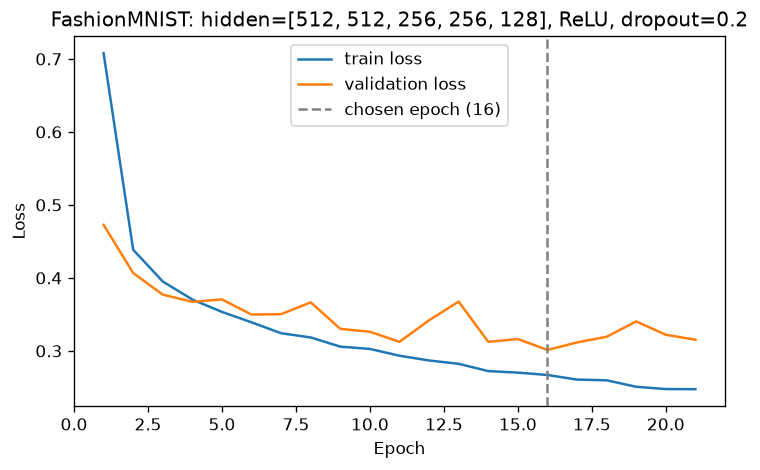
\includegraphics[width=0.7\linewidth]{figures/problem4_loss.png}
\caption{Training and validation loss versus epoch for the selected Fashion-MNIST network. The dashed line marks the chosen epoch 16, whose weights are kept; early stopping ended training at epoch 21.}
\label{fig:p4loss}
\end{figure}

\begin{table}[H]
\centering
\caption{Fashion-MNIST configurations (hidden layer sizes): epochs run before early stopping, training time (including per-epoch validation), validation accuracy and, for the selected network only, test accuracy (selected row in bold).}
\label{tab:p4}
\small
\setlength{\tabcolsep}{4pt}
\begin{tabular}{llccccc}
\toprule
Hidden layers & Activation & Dropout & Epochs & Time (s) & Val. acc. & Test acc.\\
\midrule
128 & ReLU & 0 & 23 & 12.1 & 0.8856 & --\\
256-128 & ReLU & 0 & 16 & 9.6 & 0.8912 & --\\
512-256-128 & ReLU & 0 & 16 & 10.4 & 0.8882 & --\\
256-128 & Tanh & 0 & 20 & 11.9 & 0.8904 & --\\
512-256-128-64 & ReLU & 0.2 & 18 & 13.7 & 0.8896 & --\\
512-512-256-256-128 & ReLU & 0 & 19 & 14.2 & 0.8916 & --\\
512-512-256-256-128 & ReLU & 0.2 & 21 & 17.1 & \textbf{0.8918} & \textbf{0.8857}\\
1024-512-256-128-64-32 & ReLU & 0.2 & 26 & 24.8 & 0.8874 & --\\
\bottomrule
\end{tabular}
\end{table}

\end{document}
